\section{Diagnostics, Gates, and Reporting (details)}
\label{app:diagnostics}

This appendix formalizes the diagnostics used in \CJE{}, the associated \emph{ship/stop} gates, and the reporting ledger. The main text shows a compact panel per policy; here we provide precise formulas, defaults, and recommended thresholds. Unless stated otherwise, expectations and variances are empirical over the evaluation cohort (global SNIPS normalization).

\subsection{Weight behavior \& overlap}
\label{app:diag-weights}

\paragraph{Effective sample size (ESS).}
For nonnegative weights,
\[
\ESS(W)=\frac{\big(\sum_i W_i\big)^2}{\sum_i W_i^2}.
\]
Under global mean-one normalization (SNIPS), $\sum_i W_i=n$, so
\[
\frac{\ESS(W)}{n}=\frac{1}{1+\mathrm{CV}^2(W)},\qquad
\mathrm{CV}^2(W)=\Var(W)\ \text{when }\E[W]=1.
\]
Report the \emph{ESS fraction} $\ESS(W)/n$ and the multiplicative \emph{uplift}
$\ESS(\hat W_{\pi'})/\ESS(W^{\mathrm{m1}}_{\pi'})$.

\paragraph{Max-weight share.}
$\max_i W_i \big/ \sum_j W_j$ flags single-row dominance; display alongside the empirical 99.5th percentile of $W$.

\paragraph{Tail index (Hill) and CCDF.}
For the top-$k$ order statistics $W_{(1)}\ge\cdots\ge W_{(k)}$,
\[
\hat\alpha^{-1}(k)=\frac{1}{k}\sum_{j=1}^{k}\log\!\left(\frac{W_{(j)}}{W_{(k)}}\right),\qquad k\in\mathcal{K},
\]
swept over a stability grid $\mathcal{K}$ (e.g., 1--5\% of $n$). Plot $\hat\alpha(k)$ with a band over the plateau region (median and IQR over $\mathcal{K}$), and the empirical CCDF of $W$ on a log--log scale.

\paragraph{Overlap in judge space.}
Let $p_{S|\pi_0}$ and $p_{S|\pi'}$ denote the (binned) densities of $S$ under $\pi_0$ and $\pi'$:
\[
A_B=\sum_{b}\sqrt{p_b(\pi_0)\,p_b(\pi')},\qquad D_B=-\log A_B.
\]
Overlay an $S$-binned heatmap of $\log W$ to localize regions of poor overlap.

\subsection{Judge calibration, coverage, and drift}
\label{app:diag-judge}

\paragraph{Reliability diagram.}
Partition $S$ into $B$ bins; for bin $b$, plot the bin mean of $R=\hat f(Z(S))$ against the oracle mean of $Y$, with 95\% binomial intervals. Report a Brier-style \emph{reliability} term and the OOF RMSE.

\paragraph{Coverage badge.}
Estimate the fraction of evaluation mass outside the oracle $S$ range:
\[
\texttt{OutOfRange}=\widehat{\Pr}_{\pi'}\!\big(S<S_{\min}^{\text{orc}}\ \text{or}\ S>S_{\max}^{\text{orc}}\big).
\]
Also report \emph{boundary flatness} (slope of $\hat f$ in the lowest/highest oracle decile). Large \texttt{OutOfRange} together with flat boundaries triggers \textsc{Limited Calibration Support} and the \textsc{REFUSE-LEVEL} gate.

\paragraph{Rank drift (optional anchor).}
Given a fixed anchor set of $(X,A)$ pairs scored over time, compute Kendall’s $\tau$ between historical and current judge rankings with a permutation $p$-value. Change detection on residuals can be monitored via CUSUM/EWMA with FDR control across anchors.

\subsection{DR orthogonality and decomposition}
\label{app:diag-ortho}

\paragraph{Orthogonality score.}
Let $U_i=\hat W_{\pi',i}\big(R^{\mathrm{OOF}}_i-\hat q^{\mathrm{OOF}}(X_i,A_i)\big)$ and $\bar U=n^{-1}\sum_i U_i$.
Form a Wald CI for $\bar U$ using the standard error $\sqrt{\widehat{\Var}(U)/n}$ (or a cluster-/block-robust analogue). Report $\bar U$ and its CI; near-zero indicates successful orthogonality.

\paragraph{DM--IPS decomposition.}
Display $\widehat V_{\mathrm{DM}}=n^{-1}\sum_i \hat g_{\pi'}(X_i)$ and $\widehat V_{\mathrm{Aug}}=n^{-1}\sum_i U_i$,
with CIs and the empirical correlation between their per-row contributions.

\subsection{Uncertainty: IF variance and calibration uncertainty addition}
\label{app:diag-uncertainty}
For any estimator with centered IF contributions $\{\phi_i\}_{i=1}^n$,
\[
\widehat{\Var}_{\mathrm{main}}=\frac{1}{n}\,\widehat{\Var}(\phi_i),\qquad
\widehat{\Var}_{\mathrm{total}}=\widehat{\Var}_{\mathrm{main}}+\widehat{\Var}_{\mathrm{cal}},
\]
with $\widehat{\Var}_{\mathrm{cal}}$ from the oracle jackknife (App.~\ref{app:oua}). Report the \emph{calibration uncertainty share} $\widehat{\Var}_{\mathrm{cal}}/\widehat{\Var}_{\mathrm{total}}$ and, optionally, a dependence-robust alternative (below).

\paragraph{Dependence-robust SEs.}
When time/cluster dependence is suspected, also report:
(i) \emph{cluster-robust} sandwich SEs when a cluster id (e.g., session/user) is available; and
(ii) \emph{block/stationary bootstrap} intervals (block length chosen by a simple variance-stability sweep) \citep{Kunsch1989BlockBootstrap,PolitisRomano1994StationaryBootstrap}.

\paragraph{Bootstrap with bias-corrected estimation.}
For Direct mode, we recommend bootstrap inference with $\hat\theta_{\mathrm{aug}}$ (see \cref{ssec:method-oua}). \Cref{tab:uq-diagnostics} compares UQ methods across oracle fractions, showing that bootstrap with $\hat\theta_{\mathrm{aug}}$ achieves ${\sim}$95\% coverage by correcting both variance and bias.

\begin{table}[t]
\centering
\caption{\textbf{UQ diagnostics for Direct mode.} Coverage, centering ($\bar{Z}$), and calibration (SD$(Z)$) across oracle fractions. Well-calibrated intervals have coverage $\approx 95\%$, $\bar{Z} \approx 0$, and SD$(Z) \approx 1$.}
\label{tab:uq-diagnostics}
\small
\begin{tabular}{@{}llrrr@{}}
\toprule
\textbf{Oracle} & \textbf{Method} & \textbf{Coverage} & \textbf{$\bar{Z}$} & \textbf{SD$(Z)$} \\
\midrule
\multirow{3}{*}{5\%}
& Cluster-Robust & 22\% & $+1.52$ & 9.01 \\
& Cal-Aware Jackknife & 80\% & $+0.48$ & 3.11 \\
& Bootstrap + $\hat\theta_{\mathrm{aug}}$ & \textbf{95\%} & $+0.10$ & 0.98 \\
\midrule
\multirow{3}{*}{10\%}
& Cluster-Robust & 30\% & $+1.12$ & 6.34 \\
& Cal-Aware Jackknife & 80\% & $+0.40$ & 2.52 \\
& Bootstrap + $\hat\theta_{\mathrm{aug}}$ & \textbf{96\%} & $+0.15$ & 0.98 \\
\midrule
\multirow{3}{*}{25\%}
& Cluster-Robust & 42\% & $+0.36$ & 3.46 \\
& Cal-Aware Jackknife & 84\% & $+0.18$ & 2.09 \\
& Bootstrap + $\hat\theta_{\mathrm{aug}}$ & \textbf{97\%} & $+0.08$ & 0.95 \\
\midrule
\multirow{3}{*}{50\%}
& Cluster-Robust & 56\% & $-0.07$ & 2.63 \\
& Cal-Aware Jackknife & 87\% & $-0.05$ & 1.96 \\
& Bootstrap + $\hat\theta_{\mathrm{aug}}$ & \textbf{97\%} & $+0.11$ & 0.92 \\
\bottomrule
\end{tabular}
\vspace{1mm}

\footnotesize{
$Z = (\hat\theta - \theta) / \widehat{\mathrm{SE}}$ is the normalized error.
$N{=}600$ experiments per cell (4 sample sizes $\times$ 50 seeds $\times$ 3 policies).
$\hat\theta_{\mathrm{aug}}$ corrects the plug-in bias via AIPW-style residual augmentation.
}
\end{table}


\subsection{Multiplicity for many-policy comparisons}
\label{app:diag-multiplicity}
For contrasts $\Delta_{p}=\widehat V(\pi'_p)-\widehat V(\pi^\star)$, compute Wald $p$-values and apply BH at level $q\in[0.05,0.2]$; BY can be used under strong dependence. Provide a \emph{pairwise win matrix} with FDR marks and Kendall’s $\tau$ over policy means (all policies).

\subsection{Policy-wise mean transport diagnostic}
\label{app:diag-transport}

For each target policy $\pi'$ (or more generally, each evaluation environment such as a time period or subgroup), we test whether the calibration function $f(S,X)$ learned on the base policy remains mean-unbiased.

\paragraph{Test procedure.}
Given an oracle slice under policy $\pi'$, compute the residual $\varepsilon_{\pi'} = Y - f(S,X)$ and test
\[
H_{0,\pi'}: \E_{\pi'}[\varepsilon_{\pi'}] = 0 \quad \text{vs} \quad H_{1,\pi'}: \E_{\pi'}[\varepsilon_{\pi'}] \neq 0
\]
using a one-sample $t$-test. When testing multiple policies, apply Bonferroni or BH correction across environments.

\paragraph{Interpretation (Proposition~\ref{prop:mean-transport}).}
By \cref{prop:mean-transport}, $H_{0,\pi'}$ holds if and only if the surrogate-estimated policy value equals the oracle value: $\E_{\pi'}[f(S,X)] = \E_{\pi'}[Y]$. Rejecting $H_{0,\pi'}$ implies that surrogate-only evaluation is systematically biased for policy $\pi'$: the calibration does not transport.

\paragraph{Calibration-uncertainty-corrected inference.}
To account for uncertainty in estimating $f$, the confidence interval for the mean residual should incorporate calibration uncertainty (\cref{ssec:method-oua}). In practice, we refit $f^{(-k)}$ omitting each oracle fold and compute residuals under each refit, propagating calibration uncertainty into the test statistic.

\paragraph{Actions on failure.}
If a policy fails the mean transport test:
(i) flag surrogate-only value estimates for that policy as biased;
(ii) report the estimated bias ($\hat\Delta = \bar\varepsilon_{\pi'}$) and its direction;
(iii) either recalibrate using policy-specific oracle data or fall back to oracle-only evaluation for that cell;
(iv) rankings across policies that all pass may still be valid even if absolute levels are not.

\subsection{Gates: thresholds and actions}
\label{app:diag-gates}

\begin{table}[t]
\centering
\caption{Default gates (suggested; tighten for high-stakes launches).}
\label{tab:gates}
\setlength{\tabcolsep}{4pt}
\resizebox{\linewidth}{!}{%
\begin{tabular}{llp{7.8cm}}
\toprule
\bf Gate & \bf Default & \bf Action if failed \\
\midrule
\textsc{Overlap} & $\ESS/n \ge 0.30$ (${\le}3.3{\times}$ var); Hill $\hat\alpha\ge 2$ (finite var); $A_B\ge 0.85$ ($H{\le}0.39$); TTC $\ge 0.70$ &
Use overlap weights or cohort restriction; if TTC${}<0.70$, prefer Direct over IPS; report with warning if $\hat\alpha\in[1,2)$; do not ship offline conclusions if $\hat\alpha<1$ \\
\textsc{Judge} & Reliability band covers diagonal at knots; no persistent drift alarms &
Refresh/extend oracle slice; switch to two-stage index; re-validate \\
\textsc{Identification} & \texttt{OutOfRange} $\le \eta$ (default $\eta{=}5\%$; worst-case bias ${\le}\eta$) or non-flat boundaries &
Flag \textsc{Limited Calibration Support}; set \textsc{REFUSE-LEVEL}: report rankings + partial-ID only \\
\textsc{DR} & Orthogonality CI includes $0$; no NaNs; residual tails acceptable &
Strengthen nuisances/cross-fitting; fall back to stabilized IPS as a diagnostic \\
\textsc{Multiplicity} & FDR control applied when $|\Pi'|>5$ &
Report adjusted $p$-values; avoid uncorrected winner claims \\
\textsc{Cap} & Guard rarely engaged; CI width not sensitive to $\rho$ &
If guard active on $>50\%$ folds or sensitivity high, show cap curve and prefer overlap weights/restriction \\
\bottomrule
\end{tabular}}
\end{table}

\paragraph{Threshold calibration.}
The defaults in Table~\ref{tab:gates} are operationally calibrated for typical LLM evaluation regimes ($n \approx 5{,}000$, MDE $\approx 0.02$).
Practitioners may derive context-specific values:
(i)~ESS$/n \geq f$ bounds variance inflation to $1/f$ (e.g., $f{=}0.30 \Rightarrow {\leq}3.3{\times}$);
(ii)~Hill $\alpha > 2$ ensures finite weight variance, a CLT precondition;
(iii)~$A_B$ maps to Hellinger distance via $H = \sqrt{1 - A_B}$;
(iv)~\texttt{OutOfRange}${\leq}\eta$ bounds worst-case bias by $\eta$ under bounded outcomes.
For high-stakes applications, tighten thresholds or derive them from target MDE using the CLE bound (\cref{eq:cle-bound}).

\paragraph{REFUSE-LEVEL procedure.}
When \textsc{Identification} fails: (i) gray-out level estimates; (ii) highlight \texttt{OutOfRange} and boundary flatness; (iii) report rank-only conclusions with conservative relative CIs; (iv) recommend targeted labeling in uncovered $S$ regions.

\begin{table}[t]
\centering
\caption{Assumptions Ledger: Quick Reference. For each assumption, we list the estimators it applies to, how to test it, and recommended mitigations if violated.}
\label{tab:assumptions-ledger}
\setlength{\tabcolsep}{3pt}
\resizebox{\linewidth}{!}{%
\begin{tabular}{@{}p{2.2cm}p{1.8cm}p{4.5cm}p{4.5cm}@{}}
\toprule
\textbf{Assumption} & \textbf{Applies To} & \textbf{How to Test} & \textbf{If Violated} \\
\midrule
\textbf{Overlap} (positivity) & IPS, DR & ESS$/n \geq 0.30$; Hill $\hat\alpha \geq 2$; $A_B \geq 0.85$; TTC $\geq 0.70$ & Overlap weights; cohort restriction; if TTC${}<0.70$, use Direct \\
\textbf{Transport} (T1) & All (for valid levels) & Mean residual test: $\E_{\pi'}[Y - f(S,X)] = 0$ per policy & \emph{Fundamental requirement}; test with audit; recalibrate or refuse levels if fail \\
\textbf{Mean sufficiency} (J2-M) & Reward calibration & Reliability diagram; regional residuals centered at zero & \emph{Structural}, sufficient for transport; two-stage fallback; not required if transport passes \\
\textbf{Monotonicity} in $S$ & Reward calibration & OOF RMSE comparison & Default to two-stage; use monotone-only if covariates unavailable \\
\textbf{Calibration coverage} & All & \texttt{OutOfRange} $\leq 5\%$ (worst-case bias ${\le}5\%$); non-flat boundaries & \textsc{REFUSE-LEVEL}; targeted labeling in uncovered regions \\
\textbf{Shared prompts} & Direct & Paired design check (same prompt set across policies) & Cannot use Direct; must use OPE methods \\
\bottomrule
\end{tabular}}
\end{table}

\noindent\emph{Assumption hierarchy.} Transport (T1) is the fundamental requirement for valid surrogate-only level claims. Mean sufficiency (J2-M) and Prentice-style surrogacy are \emph{sufficient conditions} that imply transport, but transport can hold without them---errors may cancel in expectation. With an audit slice, test transport directly; structural assumptions become optional. See \cref{app:assumptions-ledger} for details.

\subsection{Planner: MDE and label/log budgets}
\label{app:diag-planner}
Given two independent estimates with equal SE $\widehat{\mathrm{SE}}$, the two-sided 95\% test at 80\% power has
\[
\mathrm{MDE}_{80\%}=(z_{0.8}+z_{0.975})\sqrt{2}\;\widehat{\mathrm{SE}}.
\]
We tabulate $\widehat{\mathrm{SE}}$ versus $(n,\,m/n)$ (labels per log) using \emph{Stacked-DR} with calibration-aware variance and annotate "iso-cost'' lines for the label budget.

\subsection{Weight Stabilization Visualization}
\label{app:weight-viz}

\Cref{fig:weight-stabilization-app} illustrates the effect of weight stabilization on importance weight distributions across target policies.

\begin{figure*}[t]
  \centering
  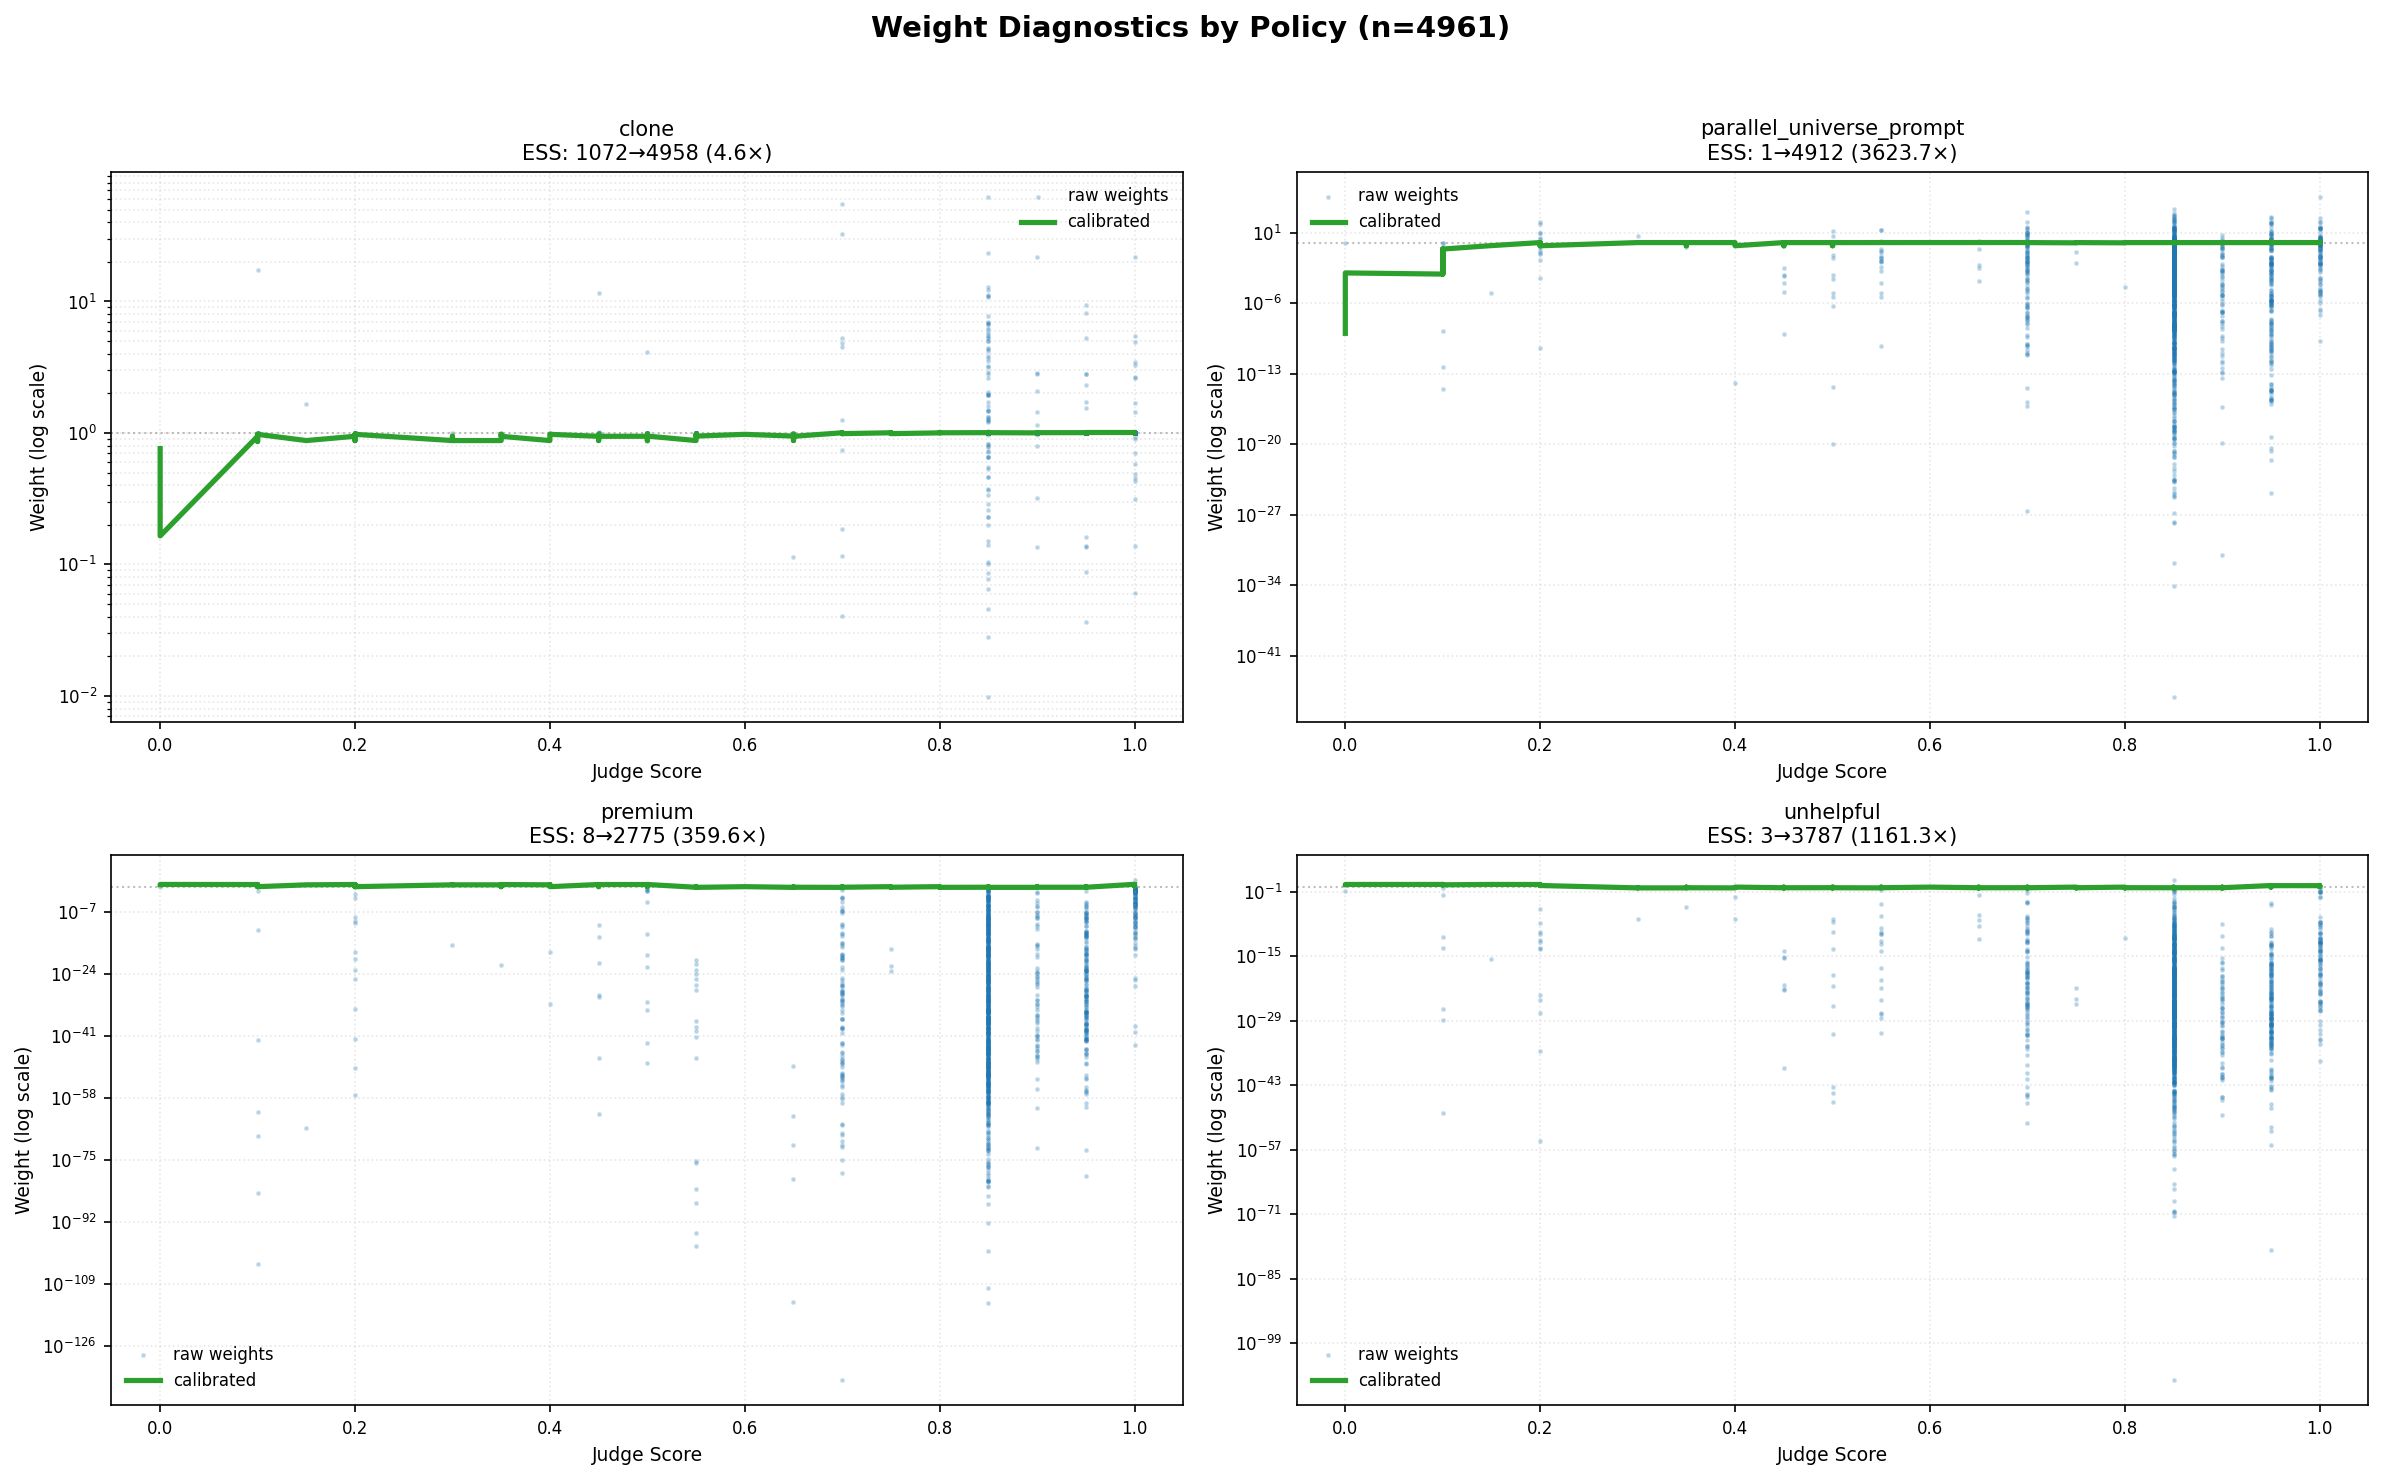
\includegraphics[width=\textwidth]{figs/weight_dashboard_per_policy.png}
  \caption{\textbf{Weight stabilization across Arena policies} ($n{=}4{,}961$ samples with complete logprobs for all four target policies). Raw importance weights (blue dots) span $10^{-130}$ to $10^{2}$; $S$-monotone projection (green line) stabilizes weights while preserving unit-mean. ESS improvements range from 4.6$\times$ (\texttt{clone}) to $>$3000$\times$ (\texttt{parallel\_universe\_prompt}). The \texttt{premium} policy shows weights spanning 130 orders of magnitude before stabilization. \textbf{Takeaway:} Weight stabilization recovers ESS from degenerate ($<$1\%) to healthy ($>$80\%), but high ESS alone doesn't guarantee ranking accuracy---coverage (TTC/CLE) is the binding constraint.}
  \label{fig:weight-stabilization-app}
\end{figure*}

\subsection{Reporting ledger (per policy/cohort)}
\label{app:diag-ledger}
Persist:
(i) calibrator mode, OOF risk by tertiles, knots/levels (hash);
(ii) weight stabilization maps, stacking weights $\hat\beta$, guard $\rho$ and blend $\alpha$;
(iii) ESS fraction, max-weight share, Hill index band, $A_B$;
(iv) DR orthogonality score and CI; DM--IPS split;
(v) calibration uncertainty trace $\{\widehat V^{(-k)}\}$ and variance breakdown;
(vi) filter counts (e.g., TF gaps) and an inclusion manifest of $x$-ids;
(vii) multiplicity control (family, $q$, adjusted $p$).

\subsection{Visualization primitives (for reproducible panels)}
\label{app:diag-viz}
\begin{itemize}[leftmargin=*,itemsep=2pt,topsep=2pt]
\item \textbf{ESS/tails strip:} bars for ESS fraction (baseline vs.\ weight stabilization); dot for max-weight share; Hill band.
\item \textbf{$S$-overlap heatmap:} density of $S$ under $\pi_0$ vs.\ $\pi'$ with overlaid $\log W$; annotate $A_B$.
\item \textbf{Reliability panel:} bin means of $(R,Y)$ with 95\% CIs; mode card (monotone vs.\ two-stage; OOF RMSE).
\item \textbf{Orthogonality panel:} point/CI for $\bar U$; DM--IPS bars with CIs and correlation.
\item \textbf{Uncertainty ring:} pie of $\widehat{\Var}_{\mathrm{cal}}/\widehat{\Var}_{\mathrm{total}}$ (calibration uncertainty share).
\end{itemize}

\subsection{Optional: dependence--robust implementation details}
\label{app:diag-dep}
\emph{Cluster-robust SEs:} if a cluster id $c(i)$ is available,
$\widehat{\Var}_{\mathrm{CR}}=n^{-2}\sum_{c}\big(\sum_{i\in c}\phi_i\big)\big(\sum_{i\in c}\phi_i\big)^{\!\top}$,
with finite-sample correction.\quad
\emph{Stationary bootstrap:} sample blocks of geometric length $\ell\sim\mathrm{Geom}(p)$ glued to length $n$; form the bootstrap distribution of $\hat\psi$ (or of $n^{-1/2}\sum\phi_i$) and report percentile or $t$-based bands.

\subsection{Compact gate pseudo-logic}
\label{app:diag-logic}
\begin{algorithm}[t]
\caption{Gate logic (per policy)}
\label{alg:gates}
\begin{algorithmic}[1]
\STATE Compute weight/tail metrics: ESS fraction, max-share, Hill band; compute $A_B$; judge reliability/coverage; orthogonality score; calibration uncertainty share
\IF{$\ESS/n<0.30$ \textbf{or} median Hill$<2$ \textbf{or} $A_B<0.85$} \STATE Flag \textsc{Overlap} (warn; restrict or use overlap weights) \ENDIF
\IF{\texttt{OutOfRange}$>\eta$ \textbf{and} boundary slopes ${\approx}\,0$} \STATE \textsc{REFUSE-LEVEL} $\leftarrow$ TRUE \ENDIF
\IF{Orthogonality CI excludes $0$} \STATE Flag \textsc{DR}; strengthen nuisances/cross-fitting \ENDIF
\IF{Cap engaged on $>50\%$ folds \textbf{or} CI sensitivity to $\rho$ high} \STATE Show cap--sensitivity; prefer overlap weights/restriction \ENDIF
\STATE Apply multiplicity control (BH/BY) when $|\Pi'|>5$
\end{algorithmic}
\end{algorithm}
